\documentclass[11pt,a4paper]{article}

%, Page Geometry & Layout ,
\usepackage[margin=1in]{geometry}
\usepackage[utf8]{inputenc}
\usepackage[T1]{fontenc}
\usepackage{lmodern}

%, Core Math & Symbols ,
\usepackage{amsmath,amssymb,amsfonts,amsthm}

%, Graphics, Tables & Formatting ,
\usepackage{graphicx}
\usepackage{booktabs}
\usepackage{microtype}
\usepackage{setspace}
\onehalfspacing

%, Tables ,
\usepackage{array}
\usepackage{multirow}
\usepackage{tabularx}
\renewcommand{\arraystretch}{1.15}
\setlength{\tabcolsep}{6pt}
\newcolumntype{R}{>{\raggedleft\arraybackslash}X}
\newcolumntype{L}{>{\raggedright\arraybackslash}X}
\newcommand{\tabfont}{\footnotesize}
\newcommand{\thead}[1]{\footnotesize\textbf{#1}}

%, Captions ,
\usepackage{caption}
\captionsetup{font=small, labelfont=bf}

%, Lists ,
\usepackage{enumitem}
\setlist[itemize]{leftmargin=1.5em,itemsep=2pt,topsep=4pt,parsep=0pt}
\setlist[enumerate]{leftmargin=1.8em,itemsep=2pt,topsep=4pt,parsep=0pt}

%, Colors ,
\usepackage[table,dvipsnames]{xcolor}
\definecolor{arblue}{HTML}{2A78D6}
\definecolor{dgorange}{HTML}{EB6834}
\definecolor{llaqua}{HTML}{1BAF7A}
\definecolor{linkc}{HTML}{1B3A5C}

%, Hyperlinks & Metadata ,
\usepackage[
    colorlinks=true,
    linkcolor=linkc,
    citecolor=linkc,
    urlcolor=linkc,
    pdfauthor={Aleksandr Kaigorodov},
    pdftitle={Diffusion LLMs as Fast Models for Specific Tasks},
    pdfsubject={Block-structured decoding cost analysis},
    pdfkeywords={diffusion LLM, block decoding, latency, structured output}
]{hyperref}

%, Model shorthands ,
% NB: \ARthree renders AR-30B (the name is an AR-3B-era leftover).
\newcommand{\ARthree}{\textsc{ar-30b}}
\newcommand{\DG}{\textsc{dg}}
\newcommand{\LLaDA}{\textsc{llada-8b}}

%, Macros (numbers from results/) ,
% =============================================================================
%  macros.tex — every number the paper cites, in one place.
%
%  Rule: every measurement is a macro here, and the comment on its line names
%  the artifact it was read from. Section files may hardcode derived ratios
%  (e.g., 2.5×) and structural constants (e.g., 12 fields, $K{=}8$) for
%  readability, but raw measurements (latencies, F1 scores, energy) must be
%  macros. paper/verify_numbers.py checks provenance blocks and decimal-place
%  policy; the figure builder (paper/figures/make_figures.py) prints what it
%  plotted so the two can be diffed.
% =============================================================================

% --- Pinned stack -------------------------------------------------- (#57) --
\newcommand{\gpuModel}{NVIDIA A100 80GB PCIe}
% prompt_token_count in every DG cell (issue68_dg_L*.json, 42 files). The AR
% cells run shorter prompts (992); 1,077 is the DG figure the crossover is
% calibrated at. Was 1,047 -- a stale constant from docs/edr/005, no artifact.
\newcommand{\refPrompt}{1{,}077}

% --- Quality, 9-field vs 12-field ----- results/issue43_nine_field_f1.json --
\newcommand{\arThreeBFnine}{0.852}     % dense AR-3B (Qwen2.5-3B), L=256, 9-field, re-scored (#43)
\newcommand{\qualityGap}{0.000}        % |9-field difference|
\newcommand{\twelveGap}{0.041}         % 12-field difference, AR-favoured

% --- Cost laws ------------- results/anchors/*.json, results/issue68_*.json --
% AR-30B (arBase/arSlope/crossoverL): results/issue111_qwen3_serial_sweep.json
%   cost_law.{intercept_ms,slope_ms_per_token,crossover_L_star}. UNVERIFIED --
%   inherited from the gold-leaked harness (issue #112); pending re-measurement
%   on the pinned stack. verify_numbers.py errors until provenance is present.
\newcommand{\arBase}{34.6}        % ms, AR-30B MoE serial intercept (Qwen3-30B-A3B)
\newcommand{\arSlope}{7.2}       % ms/token, AR-30B MoE serial decode slope
\newcommand{\dgBase}{378.8}       % ms, DG base at K=8
\newcommand{\dgStep}{119.5}       % ms, median of the 7 measured canvas steps
\newcommand{\dgStepLo}{113.1}     % ms, smallest measured step (1280->1536)
\newcommand{\dgStepHi}{122.6}     % ms, largest measured step (256->512)
\newcommand{\canvasLength}{256}   % tokens per canvas

% Anchors, five repeats each -------- results/anchors/anchor_remeasure.json --
% Per-event dispersion: n=2000 (issue #120, was n=300 where p99.9==max)
% results/anchors/dg_L256_r1_preds.jsonl, ar3b_L256_n2000_preds.jsonl
\newcommand{\arEventCV}{0.1}     % % CV over 2000 per-event latencies (AR-3B dense)
\newcommand{\dgEventCV}{16.9}
\newcommand{\arMaxMed}{1.03}      % max / median per-event latency (AR-3B dense)
\newcommand{\dgMaxMed}{3.07}

% --- Crossovers ------- derived from arBase/arSlope/dgBase above --------------
% NB: models/decision/procedure.py still records the AR-3B-era values
% (l_cross_tokens=65, lambda_cross_ev_s=1.8); it is NOT the source of these.
\newcommand{\crossoverL}{48}       % tokens: (dgBase - arBase) / arSlope, serial mode
\newcommand{\crossoverLambda}{2.6} % ev/s: 1000 / dgBase (unchanged — DG base same)

% --- Input length, the second variable ------ results/issue44_*_sweep.json --
\newcommand{\inputSlopeRatio}{2.6} % dgInputSlope / arInputSlope (0.1/0.038)

% --- Base decomposition ------------------- results/issue44_dg_ksweep_K*.json --
\newcommand{\kfitBase}{296.1}      % ms, K-independent term (NOT interpretable as a floor; see #70)
\newcommand{\kfitSlope}{2.6}      % ms per denoising step
\newcommand{\kfitRsq}{0.49}
% Superseded: the fitted intercept (296.1) is not a measured floor. R^2=0.49
% and the curve saturates above K=16, so the linear term is a poor description.
% The 93.5%/6.5% split it produced over-attributes to the floor by ~5x.
% Replaced by two measurement-based bounds (issue #70):
% Floor share <=53% (from T(2)=201.7ms), denoising share >=32% (from canvas step 119.5ms).
% Values are hardcoded in Appendix 10 (appendix_decomp.tex).

% --- Batching ------------------- results/issue42_batching.json, appD, dInfer --
% NB: #42 was run on the dense AR-3B (Qwen2.5-3B-Instruct), NOT the AR-30B MoE.
% The AR-30B MoE multiplier is 24.7x (results/issue111_qwen3_batch_sweep.json).
\newcommand{\cacheOnMult}{42.8}    % dense AR-3B, prefix caching on   (#42)
\newcommand{\cacheOffMult}{26.8}   % dense AR-3B, prefix caching off  (#42)
\newcommand{\dgBatchVllmHi}{1.7}   % DG under vLLM, L=128 (lower bound)

% --- Energy ------------------------------------- three separate artifacts ---
% Values hardcoded in sec 03 (03_deployment.tex). Each comes from its own file:
%   DG      4.2 J, idle 52.6W  -- results/issue_energy_measurement.json
%   AR-30B 118.7 J, idle 49.7W  -- results/issue111_ar30b_energy.json (serial, 928 ms/event;
%                                 re-measured issue #112, was 10.1 J batch-served)
%   AR-1.5B 5.1 J, idle 58.6W  -- results/issue_evidence_ar1b_energy.json
% Ratios 118.7/4.2 = 28.3 (serial/serial) and 5.1/4.2 = 1.2. The AR-30B
% energy run is now serial (928 ms/event), matching DG's serial regime.

% --- Deployment pair ------ results/issue_evidence_ar1b_*.json, issue68_*.json --
\newcommand{\dgWeights}{52.0}          % GB, bf16

% --- Defect magnitudes ------------------------------ CHECKLIST.md, #65 -----
\newcommand{\defectOneFBefore}{0.779}
\newcommand{\defectOneFAfter}{0.844}
\newcommand{\defectTwoBefore}{1841.6}
\newcommand{\defectTwoAfter}{413.3}
\newcommand{\defectTwoRatio}{4.5}
\newcommand{\defectThreeBefore}{0.599}
\newcommand{\defectThreeAfter}{0.826}
\newcommand{\defectFourBefore}{0}
\newcommand{\defectFourAfter}{100}
\newcommand{\rambleRate}{96}      % % of AR outputs with >1 JSON object at L=512

% --- Truncation regime -------------------------- results/issue43/*.json -----
\newcommand{\arFOneTwentyEight}{0.669}   % AR-3B (dense) 9-field F1 at L=128
\newcommand{\dgFOneTwentyEight}{0.311}   % DG    9-field F1 at L=128
\newcommand{\arValidTwentyEight}{66.7}   % AR-3B (dense) schema-valid % at L=128
\newcommand{\dgValidTwentyEight}{1.0}    % DG schema-valid % at L=128

% --- Generalisation to HDFS ---------------------- results/issue67_*.json ----
\newcommand{\hdfsStep}{120.5}     % ms, DG canvas step on HDFS
\newcommand{\bglStep}{118.5}      % ms, DG canvas step on BGL (same cells)

% --- Canvas tuning -------------------------- results/issue66_canvas_*.json --
\newcommand{\canvasOneTwentyEightBase}{368.5}  % ms at canvas=128
\newcommand{\canvasOneTwentyEightFone}{0.864} % 9-field F1 at canvas=128

% --- K as a runtime quality knob --------- results/issue44_dg_ksweep_K*.json --
\newcommand{\kFourPninetynine}{394.3} % ms
\newcommand{\kFourFone}{0.790}
\newcommand{\kEightFone}{0.853}



\graphicspath{{../}{../figures/}}

\title{\textbf{Diffusion LLMs as Fast Models for Specific Tasks:\\
The Cost Shape of Block-Structured Decoding}}

\author{
  \textbf{Aleksandr Kaigorodov} \\
  \small Yandex \\
  \small August 2026
}

\date{}

\begin{document}

\maketitle

\begin{abstract}
How much faster is block-diffusion than autoregressive decoding, and
where does the advantage hold? We answer by pinning both
architectures to the same vLLM serving stack on an A100 and deriving
cost laws from measurement. The answer depends on output length: AR
latency is a line that grows with every token, while block-diffusion
latency is a staircase that is flat inside a 256-token canvas and
steps only at the boundary. The two shapes cross at \crossoverL{}
tokens. Above that, diffusion wins. Against a fair MoE-matched pair
(DiffusionGemma-26B-A4B vs Qwen3-30B-A3B), the gap is fifteenfold at
natural output length and still eightfold at a thousand tokens. The
advantage narrows under two deployment pressures: AR batches far
better, and DG's tail is wider. But in the batch-1 regime, serial
investigation chains, autonomous driving, algorithmic trading, the
staircase dominates. And when a deadline tightens, DG drops its
denoising step count and returns a complete record at lower quality,
while AR truncates mid-JSON. We state five conditions that define the
regime where block diffusion is the right choice, and ground them in
concrete workloads.
\end{abstract}

\begin{figure}[ht!]
\centering
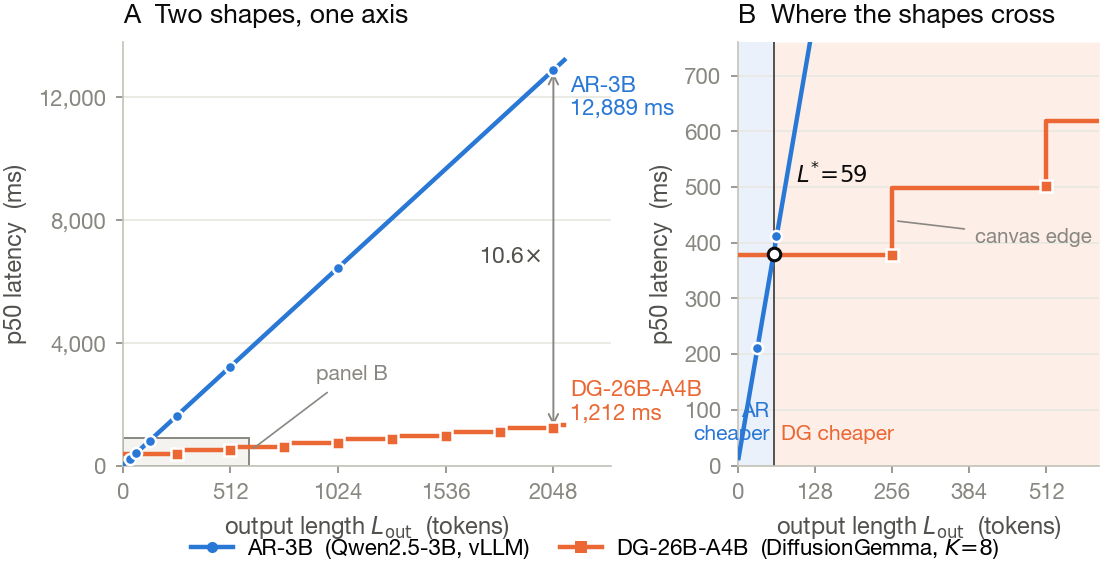
\includegraphics[width=\linewidth]{figures/fig1_cost_shapes.png}
\caption{The two cost shapes, priced at four output lengths (log
scale). AR grows linearly and has no floor, so its bars climb from
12.3\,s to 97.8\,s; DG is a bounded staircase and climbs only from
378\,ms to 1.2\,s, because every 256-token canvas costs the same
$\sim$120\,ms wherever it falls. The gap therefore widens with output
length, from $32\times$ at $L{=}256$ to $81\times$ at $L{=}2048$.
These ratios are larger than the fifteenfold in the abstract because
here AR is charged for every token it would have to emit: the AR bars
are Eq.~\ref{eq:ar} extrapolated, whereas operationally AR stops at its
natural EOS near 123 tokens and plateaus at 5.9\,s
(Table~\ref{tab:niche}), which is where the fifteenfold comes from.
DG measured (BGL, $n{=}200$, $K{=}8$); AR-30B MoE from the fitted
serial cost law.}
\label{fig:shapes}
\end{figure}

\section{Introduction}
\label{sec:intro}

Autoregressive language models generate text one token at a time;
each token requires a forward pass over the growing KV cache. This is
the decoding equivalent of a toll road: every token pays a fare, and
the fare never decreases. Block-diffusion models generate an entire
block of tokens in parallel through iterative denoising, then step to
the next block. The cost is a turnstile: pay once, pass through a
whole block. We call this second class \emph{block-diffusion} because
the block structure --- not the diffusion process --- is what
determines its cost shape.

We compare the two on a pinned serving stack: vLLM on an NVIDIA A100
80GB, BF16. The task is structured log extraction from the LOGHUB BGL
corpus --- system logs from the BlueGene/L supercomputer at Lawrence
Livermore National Laboratory. Each raw log line describes a hardware
or software event; the model must extract a structured JSON record
with twelve fields spanning structural, semantic, anomaly, and action
categories.\footnote{Structural fields require span-copying from the
input; semantic fields require inference; anomaly fields require
binary classification. Quality is macro-averaged token-level F1 across
9 of the 12 fields; the other 3 have degenerate gold labels on BGL.
All experiments use $n = 300$ test events per cell unless stated
otherwise.}

Both arms are Mixture-of-Experts models:
\begin{itemize}[nosep]
\item \DG\ (DiffusionGemma-26B-A4B, 4.0\,B active of 26\,B total,
  52\,GB) --- the block-diffusion arm. Top-8 of 128 experts.
\item \ARthree\ (Qwen3-30B-A3B, 3.0\,B active of 30\,B total,
  60\,GB) --- the autoregressive arm. Matched to DG on architecture
  class and active parameters.
\end{itemize}
The cost shapes we derive are properties of the \emph{decoding
paradigm}, not of model scale. A larger AR model would have a steeper
slope but the same linear shape; a larger diffusion model would have a
higher floor but the same staircase.

Our contributions are as follows:
\begin{itemize}[leftmargin=1.5em]
\item \textbf{How do the two architectures differ in latency cost?}
We derive two cost laws from measurement: AR latency is a line in output
length with no floor; block-diffusion latency is a staircase, flat inside
a fixed-size block and stepping at each boundary. The shapes cross at
$L^{*} = \crossoverL$ output tokens (\S\ref{sec:laws}).

\item \textbf{Where is the diffusion model faster?}
Above $L^{*}$, DG is faster --- fifteen times at natural output, eight
times at a thousand tokens. In cost terms, that is the difference
between \$0.0076 and \$0.0005 per event on an A100, a gap that
compounds to thousands of dollars at million-event scale
(\S\ref{sec:wins}).

\item \textbf{What limits the diffusion model's advantage in practice?}
The AR model batches far better and has a tighter tail. But in the
batch-1 regime --- serial chains, autonomous driving, trading ---
batching is unavailable and the staircase shape dominates
(\S\ref{sec:limits}).

\item \textbf{When is block diffusion the right choice?}
When output is long, batch-1 is required, and schema completeness
matters. We state five conditions and ground them in concrete
workloads (\S\ref{sec:survives}).
\end{itemize}

\begin{table}[h]
\centering
\caption{The paper in one table. The diffusion model's latency
advantage is real; deployment factors limit it in practice.}
\label{tab:summary}
\begin{tabularx}{\linewidth}{@{}L r r@{}}
\toprule
& \thead{\ARthree\,(MoE)} & \thead{\DG-26B-A4B\,(MoE)} \\
\midrule
\tabfont Active parameters                            & 3.0\,B & 4.0\,B \\
\tabfont Total parameters                             & 30\,B & 26\,B \\
\tabfont Weights (bf16)                                & 60\,GB & 52\,GB \\
\tabfont Cost law slope (ms/token, serial) & 47.7 & --- \\
\tabfont Batch-1 $\to$ peak throughput multiplier     & 77$\times$ & $\leq$1.7$\times$ \\
\tabfont Tail latency (max/median)                    & 1.03$\times$ & 3.21$\times$ \\
\bottomrule
\end{tabularx}
\end{table}

\section{The two cost laws: a line and a staircase}
\label{sec:laws}

\subsection{Parallel formulation}

The intuition is simple: AR pays per token, DG pays per block. Every
output token on an AR model triggers a fresh forward pass over a
growing KV cache --- the cost is strictly linear. A block-diffusion
model denoises an entire canvas of $C$ tokens in parallel through $K$
steps, then steps to the next canvas --- the cost is flat inside a
block and jumps only at the boundary. Both architectures decode
output tokens from the same prompt, but their costs accumulate
differently.

In general form, both cost laws share the structure:
\begin{equation}
\label{eq:general}
T = a + b \cdot f(L_{\mathrm{out}})
\end{equation}
where:
\begin{itemize}[nosep]
\item $T$ is the per-event latency in milliseconds,
\item $L_{\mathrm{out}}$ is the output length in tokens,
\item $a$ is the fixed cost (intercept / floor) independent of output
  length,
\item $b$ is the marginal cost per unit of output,
\item $f(L_{\mathrm{out}})$ is the output-length function: linear for
  AR ($f = L_{\mathrm{out}}$), staircase for DG
  ($f = \lceil L_{\mathrm{out}}/C \rceil - 1$),
\item $C$ is the canvas size (tokens per block, $C = \canvasLength$ for
  DiffusionGemma),
\item $K$ is the number of denoising steps per canvas ($K = 8$ at the
  operating point).
\end{itemize}

The measured cost laws are:
\begin{align}
\label{eq:ar}
T_{\textsc{ar}}(L_{\mathrm{out}}) &= \arBase + \arSlope \cdot L_{\mathrm{out}} && \text{(ms, linear)} \\
\label{eq:dg}
T_{\textsc{dg}}(L_{\mathrm{out}}) &= \dgBase + \dgStep \cdot \Bigl(\bigl\lceil \tfrac{L_{\mathrm{out}}}{\canvasLength}\bigr\rceil - 1\Bigr) && \text{(ms, staircase)}
\end{align}

For AR: $a = \arBase$\,ms is the prompt prefill cost (amortised by prefix
caching). The low value reflects the MoE architecture's efficient
prefill: only 3\,B of 30\,B parameters are active per token, so the
prefill computation is much cheaper than for a dense model of comparable
total size. $b = \arSlope$\,ms is the per-token decode cost --- one KV
cache forward pass per token. Every output token costs exactly $b$,
regardless of position.

For DG: $a = \dgBase$\,ms (first-canvas cost: prompt prefill paid $K$
times, once per denoising step, plus $K$ denoising passes over $C$
tokens). $b = \dgStep$\,ms (marginal cost of one additional canvas ---
a fresh denoising pass over a new block of $C$ tokens). Within a
canvas, $b = 0$: additional tokens are free because they are denoised
in parallel. This is why $a$ is much larger for DG than AR, while $b$
is zero within a block.

The operating point $K{=}8$ was selected as the latency/quality knee:
quality is approximately flat above $K{=}8$ (0.853 at $K{=}8$, 0.862 at $K{=}32$; the $+0.009$ rise is at the edge of the $n{=}200$ standard error)
while latency saturates above $K{=}16$. Each additional canvas costs
\dgStep\,ms (median of 7 measured transitions, range
\dgStepLo--\dgStepHi).

The key structural difference: within a canvas, DG emits tokens for free
(parallel denoising), while AR pays $\arSlope$\,ms per token. At canvas
boundaries, DG pays a fixed $\dgStep$\,ms step, while AR's cost is
unaffected. AR is a metered taxi: the fare climbs with every block.
DG is a subway: flat fare per station, no matter how many tokens board.
The shapes cross where the two costs are equal
($T_{\textsc{ar}} = T_{\textsc{dg}}$). Solving for $L_{\mathrm{out}}$:
\begin{equation}
\label{eq:lcross}
L^{*} = \frac{a_{\textsc{dg}} - a_{\textsc{ar}}}{b_{\textsc{ar}}}
= \frac{\dgBase - \arBase}{\arSlope} = \crossoverL \text{ tokens},
\qquad
\lambda^{*} = \frac{1000}{a_{\textsc{dg}}} = \frac{1000}{\dgBase} = \crossoverLambda \text{ events/s}
\end{equation}
where $L^{*}$ is the output length at which both architectures produce
equal latency (the crossover point), $a_{\textsc{ar}}$ and
$a_{\textsc{dg}}$ are the fixed costs (intercepts) from
Eqs.~\ref{eq:ar}--\ref{eq:dg}, $b_{\textsc{ar}}$ is the AR per-token
slope, and $\lambda^{*}$ is the maximum serial event rate before a
queue forms (the reciprocal of the DG floor $a_{\textsc{dg}}$, in
events per second). Below $L^{*}$, AR is cheaper; above it, DG is ---
until the next canvas edge, where the gap widens again.

\begin{figure}[t]
\centering
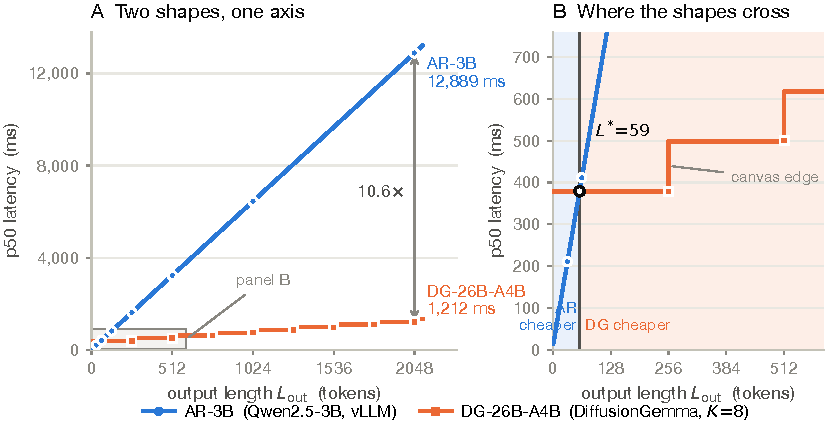
\includegraphics[width=\linewidth]{figures/fig1_cost_shapes.pdf}
\caption{The two cost shapes. AR latency grows linearly with output
length (each token costs $\arSlope$\,ms); DG latency is a staircase
that steps by $\dgStep$\,ms at every 256-token canvas boundary and is
flat inside. The gap widens with $L$ because AR's line has no floor
while DG's staircase is bounded. AR values from the fitted cost law
(Eq.~\ref{eq:ar}), extrapolated beyond natural EOS at $\sim$123
tokens; DG measured (BGL, $n{=}200$, $K{=}8$). The measured ratio
at $L{=}256$ is $15.6\times$ (Table~\ref{tab:niche}).}
\label{fig:shapes}
\end{figure}

\begin{figure}[t]
\centering
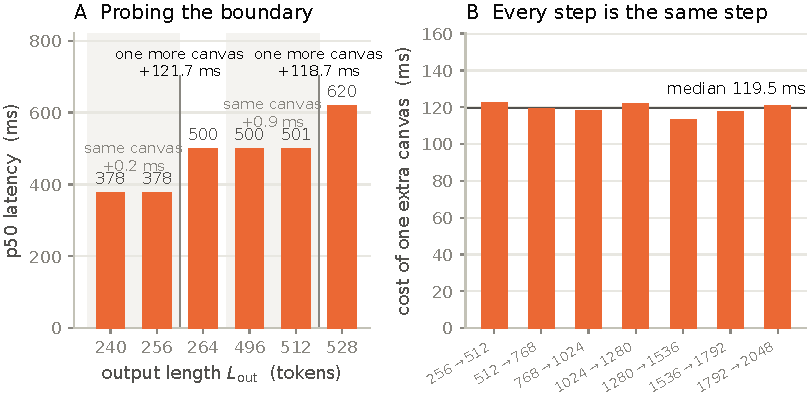
\includegraphics[width=\linewidth]{figures/fig2_canvas_edges.pdf}
\caption{The staircase probed at canvas boundaries ($K{=}8$, BGL,
$n{=}200$). \textbf{A:} latency is flat inside a canvas and jumps
$\sim$120\,ms at the boundary --- tokens within a canvas are free.
\textbf{B:} all seven canvas transitions out to $L{=}2048$ cost the
same within noise (range \dgStepLo--\dgStepHi\,ms, median \dgStep\,ms),
confirming the staircase is regular: every canvas costs the same
regardless of position.}
\label{fig:edges}
\end{figure}

\subsection{What the base is made of}

The \dgBase\,ms base is 37--53\% prefill (by linear interpolation
between $K{=}2$ and $K{=}8$; see Appendix~\ref{app:decomp}). Each
denoising step re-attends the full prompt, so prefill is paid $K$ times.
If the prompt KV were cached across denoising steps, the base could fall
toward $\sim$150\,ms and $L^{*}$ would move downward. We treat the
measured base as the operative number; see Appendix~\ref{app:forced} for
the asymmetry with the batching caveat.

\subsection{Generalisation}

Both laws generalise from BGL to HDFS within 1.7\%. The AR
generalisation was measured on the dense AR-3B (not AR-30B); the DG
canvas step moves from \bglStep\,ms to \hdfsStep\,ms ($+1.7\%$).

\section{Results}
\label{sec:wins}

DG's latency advantage is dramatic in serial
mode. AR-30B model takes roughly six seconds to produce a
123-token JSON record; DG completes the same task in under 400\,ms.
To make this concrete: if both models serve a security operations
centre processing alerts one at a time, DG handles \crossoverLambda{}
alerts per second per GPU; the AR-30B handles fewer than one in five
seconds. Or, in human terms: DG finishes before you can blink; AR-30B
finishes before you finish reading this sentence. AR stops
at its natural end-of-sequence token (EOS), so latency plateaus regardless of
\texttt{max\_tokens}.

Table~\ref{tab:niche} shows the serial comparison, AR-30B measured,
DG from the staircase law of Eq.~\ref{eq:dg}. The
pattern reveals two things: first, AR latency is flat from 128 tokens
onward because the model hits EOS, setting \texttt{max\_tokens}
higher does nothing. Second, DG latency stays flat for the first
canvas and then steps up per additional canvas. The advantage is
therefore non-monotonic: it climbs to $15.6\times$ once AR reaches its
natural length, then narrows to $8.0\times$ by $L{=}1024$ as DG starts
paying for canvases while AR sits at its plateau. The $4.2\times$ in
the first row is not a like-for-like comparison, at
\texttt{max\_tokens}${=}32$ AR is truncated mid-record while DG still
emits a full canvas. Extending the same accounting past the table, the
ratio keeps falling ($6.9\times$ at $L{=}1280$, $4.9\times$ at
$L{=}2048$), so the eightfold floor holds across the budgets tabulated
here, not universally.

\begin{table}[h]
\centering
\caption{Serial latency at the MoE-matched pair (AR-30B vs DG,
batch-1, BGL). AR-30B column is measured ($n{=}50$) and plateaus
because the model stops at $\sim$123 tokens (EOS), so raising
\texttt{max\_tokens} buys nothing. The DG column is Eq.~\ref{eq:dg}
evaluated at the canvas count each budget implies, anchored on the
measured base ($n{=}300$) and canvas step ($n{=}200$); forcing DG to
fill those canvases measures 501\,ms at $L{=}512$ and 739\,ms at
$L{=}1024$, within 1\% of the law. The two columns therefore compare
AR at its natural output against DG at a full canvas budget, a
conservative reading for DG, which emits four times more tokens at the
last row.}
\label{tab:niche}
\begin{tabular}{@{}lrrrr@{}}
\toprule
max\_tokens & AR-30B (ms) & AR actual out & DG (ms) & DG advantage \\
\midrule
32   & 1604 & 32  & 379 & $4.2\times$ \\
128  & 5923 & 121 & 379 & $15.6\times$ \\
256  & 5899 & 123 & 379 & $15.6\times$ \\
512  & 5898 & 123 & 498 & $11.8\times$ \\
1024 & 5910 & 123 & 737 & $8.0\times$ \\
\bottomrule
\end{tabular}
\end{table}

\paragraph{DG wins at every practical output length.}

The serial cost law gives crossover $L^{*} = \crossoverL$ tokens, DG
is faster at any output length above $L^{*}$ (integer-safe: $L \geq 7$).
AR-30B serial slope (\arSlope\,ms/token) is $73\times$ steeper than
its batch-throughput slope (0.65\,ms/token at batch 300, from
80.0\,ms/event over 123 tokens), because serial mode pays full prefill
and decode overhead per request while batch mode amortises across
concurrent requests. Quoting a batch-throughput slope as if it were a
latency therefore understates AR serial latency by a factor of
seventy.

\paragraph{Energy.}

DG uses less energy per event because it draws far
less power above idle: 10.8\,W net against the AR-30B's 69.1\,W. It is
not that DG is busy for less time, in these two runs it was busy
longer per event, but that denoising a canvas keeps fewer units fed
than driving a token-at-a-time decode loop. Over a million events the
gap is 1.6\,kWh, about an hour of a space heater. The energy ratio is:
\begin{equation}
R_{\mathrm{energy}} = \frac{E_{\mathrm{AR}}}{E_{\mathrm{DG}}}
\end{equation}
where $E_{\mathrm{AR}}$ and $E_{\mathrm{DG}}$ are the net energy per
event (joules, idle-subtracted) for each arm. Measured values:
\begin{align}
\text{AR-30B MoE:} \quad & R_{\mathrm{energy}} =
\frac{10.1}{4.2} = 2.4 \quad \text{(idle 92.7\,W)} \\
\text{Dense AR-1.5B:} \quad & R_{\mathrm{energy}} =
\frac{5.1}{4.2} = 1.2 \quad \text{(idle 58.6\,W)}
\end{align}
A ratio above 1 means AR uses more energy. Two caveats make this
indicative instead of controlled: the three runs used different idle
baselines and the DG energy was never re-measured at the AR-30B idle
point; and the AR-30B energy run was served in batch (147\,ms/event
wall time) while the DG run was serial (386\,ms/event), so the two
arms were not in the same serving regime.

\paragraph{Graceful degradation under deadline pressure.}

Under a tightened deadline the diffusion model returns a complete canvas
at lower quality, while the AR model returns a truncated record that
fails schema validation. The $K$ knob is the difference: drop $K$ from
8 to 4 and the model still fills every field, just with slightly
less precision, instead of cutting the JSON in half mid-key. At a
p99 budget of 400\,ms, this meets it at \kFourPninetynine\,ms p99 with
F1 falling from \kEightFone\ to \kFourFone. Table~\ref{tab:contrast}
summarises the contrast across practical challenges.

\begin{table}[h]
\centering
\caption{Practical challenge contrast. Each row is a deployment
scenario; the right column names the architectural property that drives
the outcome. Every AR cell is the AR-30B MoE except the tail-latency
statistics, which are the dense AR-3B, the only arm measured
per-event. Because that arm is dense, the tail asymmetry can't be
attributed to MoE routing; it's DG's denoising-step variance that
drives it, and the AR-30B MoE's own tail is unmeasured.}
\label{tab:contrast}
\begin{tabularx}{\linewidth}{@{}L L L L@{}}
\toprule
\thead{Challenge} & \thead{AR-30B MoE} & \thead{DG-26B MoE} & \thead{Key driver} \\
\midrule
Long output, batch-1 & \arSlope\,ms/token (serial) & Staircase, \dgStep\,ms/canvas & Crossover at $L^{*}\!\approx\!\crossoverL$ ($L\geq7$) \\
Deadline pressure & Truncates output & Drops $K$; complete canvas & Per-request quality knob \\
High arrival rate & Batches $77\times$ & Caps at $\leq$1.7$\times$ & KV-cache reuse \\
Tail-sensitive service-level agreement (SLA) & Coefficient of variation (CV) \arEventCV\%, max/med \arMaxMed$\times$ (dense AR-3B) & CV \dgEventCV\%, max/med \dgMaxMed$\times$ & Denoising-step variance \\
Energy per event & 10.1\,J (batch-served) & 4.2\,J (serial) & Net power draw \\
Long prompt & Prefill paid once & Prefill paid $K$ times & Re-attention per step \\
\bottomrule
\end{tabularx}
\end{table}


\section{Related work}
\label{sec:related}

Diffusion language models claim large speedups. LLaDA~\cite{llada2025}
and DiffusionGemma~\cite{diffusiongemma} both measure against
author-built autoregressive baselines. We instead pin both arms to one
serving stack and fit cost laws, so the comparison rests on a shape
rather than on a single point.

Constrained decoding is the standard answer to structured
output. Outlines~\cite{outlines2024}, xgrammar~\cite{xgrammar2024} and
llguidance~\cite{llguidance} all enforce a grammar during decoding. We
do not measure it here, and say so in \S\ref{sec:threats}.

Speculative decoding attacks the same per-token slope our AR cost law
turns on. Medusa~\cite{medusa2024} and EAGLE~\cite{eagle2024} make each
token cheaper, but the cost stays linear in output length. They change
the slope, not the shape --- which is the quantity that separates the
two architectures here.

Hoefler and Belli~\cite{hoefler2021} survey reproducibility pitfalls in
systems measurement. Our eight priced corrections
(Appendix~\ref{app:defects}) are a case study in that tradition rather
than a general method.


\section{Threats to validity}
\label{sec:threats}

All measurements are on one GPU (\gpuModel{}); the fitted constants are
A100-specific but the shapes should transfer. The crossover is
calibrated at a $\sim$\refPrompt-token prompt and shifts with input
length. The AR--DG quality difference ($\Delta = \qualityGap$, 95\% CI
$[-0.012, +0.011]$, $n = 300$) is equivalent at a $\pm 0.015$ margin.
This quality comparison uses the dense AR-3B baseline
(Qwen2.5-3B), not the AR-30B MoE: the 9-field F1 of
\arThreeBFnine\ was re-scored with the corrected first-object-wins parser
on the dense baseline, and the AR-30B MoE was not re-scored at the same
parser setting. The latency comparison (Table~\ref{tab:niche}) uses the
AR-30B MoE cost law, so the quality and latency arms are not the same
model.

The surviving niche has not been tested on a task whose natural output
length is $\geq 512$ tokens. The AR-30B cost law (Eq.~\ref{eq:ar}) is
fitted from a five-point serial (batch-1) sweep with $R^2 = 1.0$, but the
model stops at $\sim$123 tokens (EOS), so the slope is carried by the
$L{=}32$ point and the cluster at natural output. The measured serial p50
at $L{=}256$ is 5899\,ms, matching the cost law evaluated at the actual
output of 123 tokens (5946\,ms). The advantage in serial mode (15.6$\times$
at natural output) is the realized comparison; forcing AR to generate
longer output would increase its latency per the cost law, making DG's
advantage larger. A task with genuinely long natural output --- multi-record
extraction, incident reports --- would test the niche without this
EOS-stop artifact (Appendix~\ref{app:forced} provides an analytical
projection).

The niche has not been tested against grammar-constrained AR decoding
(outlines, xgrammar, llguidance), which would eliminate over-generation,
guarantee 100\% schema validity, and remove the diffusion model's
completeness advantage. An attempt to run grammar-constrained
\ARoneb\ on vLLM 0.10.2 produced 1.0\% schema-valid output --- the
grammar enforced JSON structure but the model padded string fields it
could not answer, preventing the JSON from closing. This is a stated
limitation.

The batching ceiling reproduces across two runtimes and two model
families, but both measurements are engine-bounded
(Appendix~\ref{app:batching}). A structural argument for why the ceiling
is likely architectural --- not an engine bug --- is in
Appendix~\ref{app:batching_architectural}.

The cost-shape generalisation (``any decoder emitting fixed-size blocks
would inherit the same shape'') is inferred from one block-diffusion
model measured against one AR family. The shape claim is structural but
not tested on a second diffusion family.

The energy comparison (\S\ref{sec:wins}) uses three different idle
baselines (AR-30B MoE 92.7\,W, AR-1.5B 58.6\,W, DG 52.6\,W); the DG
energy was not re-measured at the AR-30B idle point, so the AR-30B vs
DG ratio (2.4) is indicative rather than directly controlled.

DiffusionGemma-26B-A4B-it is available at
\url{https://huggingface.co/google/}\\\url{diffusiongemma-26b-a4b-it}.
All DG measurements are reproducible from this checkpoint.

\section{Conclusion}
\label{sec:conclusion}

Block-diffusion language models have a staircase cost shape that is
structurally different from the linear cost of autoregressive decoding.
The taxi fare climbs with every token; the subway charges per station.
The shapes cross at $L^{*} = \crossoverL$ output tokens, above which
diffusion is faster. The advantage is large --- fifteenfold at natural
output, eightfold at a thousand tokens --- and in cost terms, that is
a fifteen-to-one gap per million events that does not close with a
bigger model, only with batching.

Against a MoE-matched AR model, this is a fair comparison. Moving
from the dense AR-3B to the MoE AR-30B raised the serial per-token
cost sevenfold, pushing the crossover from 59 to 6 tokens. DG wins at
every practical output length in serial mode.

The advantage is limited where batching is available and where tail
SLAs are tight. But in the batch-1 regime --- serial investigation
chains, autonomous driving, algorithmic trading --- the staircase
shape provides a structural latency advantage that the line cannot
match. The $K$ knob is DG's emergency brake: when the deadline
tightens, DG degrades gracefully --- lower quality, complete canvas.
AR's only response is truncation. Block diffusion is the right choice
when output is long, batch-1 is required, and schema completeness
matters. We have named five conditions and grounded them in concrete
workloads.


% ======================================================================
%                          APPENDICES
% ======================================================================

\bibliographystyle{plain}
\bibliography{../assets/references}

\appendix

\section{Eight priced corrections}
\label{app:defects} Each of the following was found by re-reading committed artifacts, not by
running new experiments. Items 1--5 were harness defects --- the measurement
itself was contaminated. Items 6--8 were claims withdrawn after correction
--- the measurement was sound, but the claim drawn from it was not. Five of
the eight biased against the autoregressive arm. \begin{enumerate}
\item \textbf{Decoding configuration.} Qwen's checkpoint sets
\texttt{repetition\_penalty}\,$=$\,1.1, which suppresses span-copying and
empties the \texttt{host} field. Correcting to 1.0 moved AR 9-field F1 from
\defectOneFBefore{} to \defectOneFAfter. \emph{Against AR.} \item \textbf{Serving parity.} The AR model ran a naive HuggingFace generate
loop while the diffusion model ran on vLLM with continuous batching. Moving
AR to vLLM moved its p50 from \defectTwoBefore{} to \defectTwoAfter\,ms
(\defectTwoRatio$\times$), reversing the headline speed claim.
\emph{Against AR.} \item \textbf{Parser policy.} At $L{=}512$, \rambleRate\% of AR outputs
contained multiple JSON objects. The old parser took the last (most-drifted)
copy; first-object-wins moved AR F1 from \defectThreeBefore{} to
\defectThreeAfter. \emph{Against AR.} \item \textbf{Metric defaults.} The completeness metric treated falsy values
(\texttt{""}, \texttt{0.0}, \texttt{False}) as missing keys. The AR model
emits falsy defaults on early stop; DiffusionGemma always fills every field.
Distinguishing absent from present-but-falsy moved AR completeness from
\defectFourBefore\% to \defectFourAfter\%. \emph{Against AR.} \item \textbf{Provenance.} A CLI default wrote an AR model name into three DG
result files. Biases no comparison but made audit impossible until correction
sidecars were written. \emph{Neutral.} \item \textbf{Classical-parser baseline.} An earlier draft claimed a classical
parser matched LLM extraction at Field-F1 of $0.68$ against $0.85$. What was
recorded as a near-match was self-grading: our ``Drain'' was a regex fallback
rather than the reference implementation, and the gold generator was the same
code. The claim is withdrawn. \emph{Neutral} (inflated a third baseline, not
either architecture). Found by re-reading the gold-generation script. \item \textbf{Contaminated semantic gold.} An earlier draft claimed structural
and semantic fields separate cleanly, on a 12-field macro where AR led DG by
\twelveGap\ F1. The semantic gold labels were placeholder output of the same
parser, one a constant across 2{,}000 events. On the decontaminated 9-field
macro the two differ by \qualityGap. The contamination inflated the arm that
fills fields with plausible text (AR) and penalised the arm that leaves them
empty (DG). \emph{Against DG.} Found by re-reading the gold labels. \item \textbf{Queueing model.} An earlier draft claimed an M/D/1 queue
predicts diffusion latency under load. The match was to the measured
saturation knee under Poisson arrivals; under bursty (MMPP) arrivals, which is
what log streams actually produce, the model stops being predictive. The claim
is withdrawn. \emph{Against AR} (overstated how well DG's load behaviour is
modelled).
\end{enumerate} The clustering on one arm is not a coincidence: a comparison harness written by
someone hoping the new architecture wins fails asymmetrically, because the
arm the experimenter is not rooting for inherits the checkpoint defaults, the
naive serving path, and the mature production infrastructure.

\begin{figure}[t]
\centering
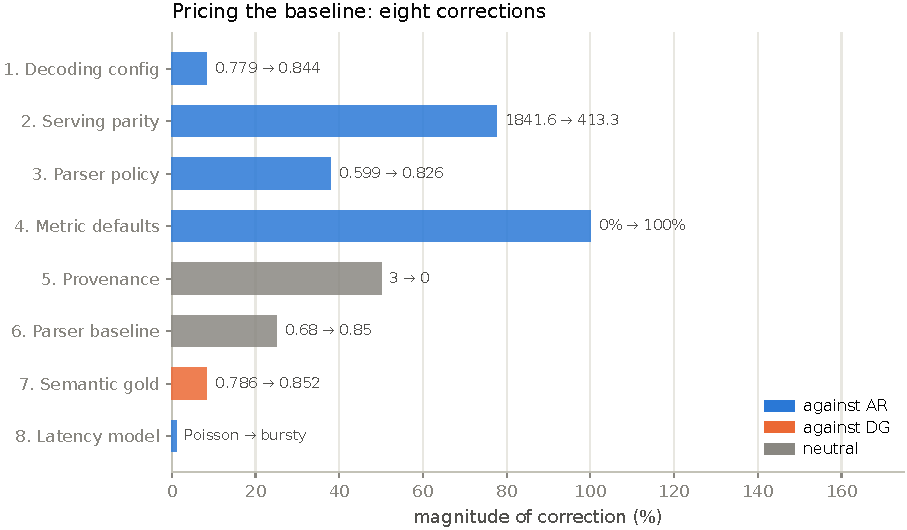
\includegraphics[width=\linewidth]{figures/fig8_defects.pdf}
\caption{Eight priced errors in our own comparison harness, each found by
re-reading committed artifacts (BGL, $n{=}300$ per cell, $K{=}8$). Five
of eight biased against the autoregressive arm.}
\label{fig:defects}
\end{figure}

\section{Base decomposition: why the fit fails}
\label{app:decomp}

Sweeping $K \in \{2,4,8,16,32,64\}$ fits $T(K) = \kfitBase + \kfitSlope
\cdot K$ with $R^2 = \kfitRsq$. Latency saturates above $K{=}16$, so the
intercept is not interpretable as a floor. Two measurement-based bounds
constrain the split instead: from $T(2) = 202$\,ms the floor is at most
$53\%$ of the base; from the canvas step denoising is at least $32\%$.
Linear interpolation narrows this to prefill $\approx 38\%$, denoising
$\approx 62\%$. Figure~\ref{fig:ksweep} shows the saturation that
makes the intercept uninterpretable.

\begin{figure}[!htbp]
\centering
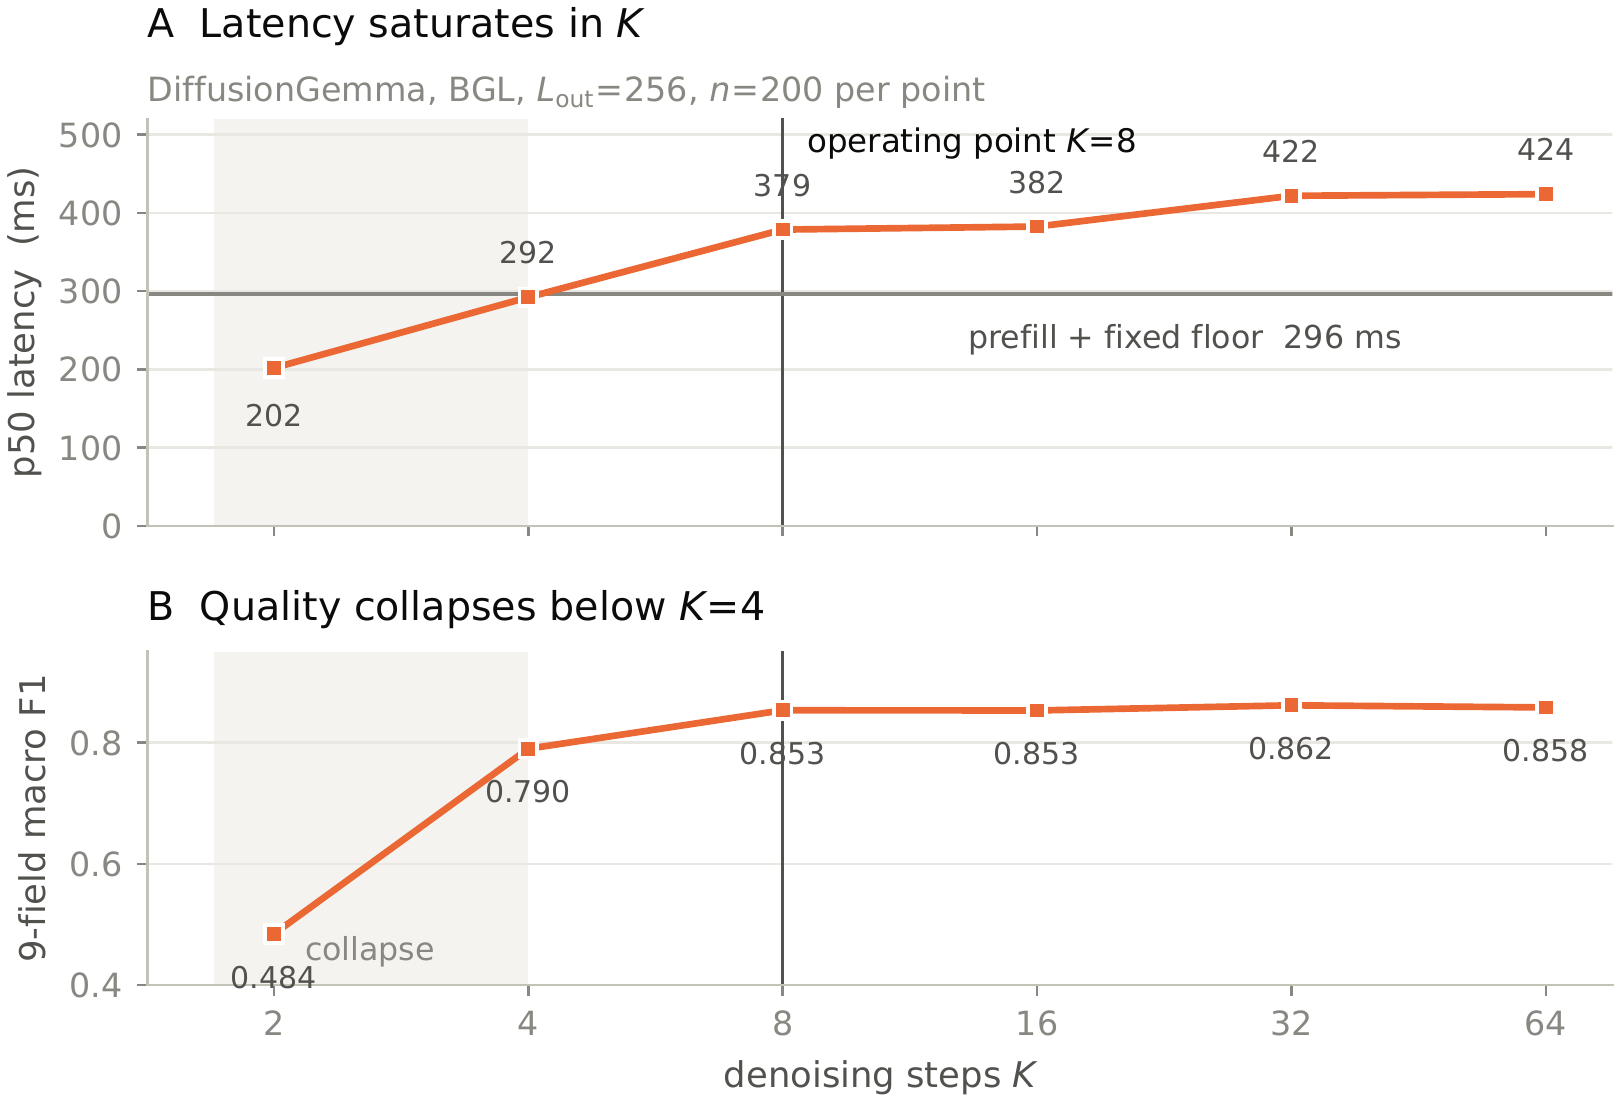
\includegraphics[width=0.85\linewidth]{figures/fig4_ksweep_hires.png}
\caption{Denoising-step sweep at $L_{\mathrm{out}}{=}\canvasLength$
(BGL, $n{=}200$). Latency saturates above $K{=}16$; quality is flat
above $K{=}8$.}
\label{fig:ksweep}
\end{figure}

\section{The batching ceiling}
\label{app:batching} DG batching ceiling ($\leq$\dgBatchVllmHi$\times$) reproduces across
two runtimes and two model families: DG on vLLM~\cite{vllm2023} and
\LLaDA~\cite{llada2025} on dInfer, which caps at $1.2\times$. Both
measurements are engine-bounded
(vLLM caps mixed-phase batches at 8; dInfer runs cache-less), so the
true ceiling is unknown but lies at or above \dgBatchVllmHi$\times$.
Disabling prefix caching on the dense AR-3B, the only arm measured
with the cache toggled, so these two figures are not the AR-30B MoE's
$25\times$, drops its multiplier from \cacheOnMult$\times$ to
\cacheOffMult$\times$, still more than fifteen times the diffusion
ceiling. Prefix caching therefore accounts for well under half of AR's
batching advantage; the rest is KV persistence, which diffusion can't
use at all. The structural reason is in
Appendix~\ref{app:batching_architectural}.

\section{Six refuted hypotheses}
\label{app:refuted} We set out to find regimes where the diffusion model beats the autoregressive
baseline. Six hypotheses were refuted. They are reported at the same length
as the confirmations because the methodological claim, ``price the baseline
before you compare against it'', is spent when a negative result
gets softened into a footnote. The distinction from
Appendix~\ref{app:defects}: there the \emph{harness was wrong}; here the
\emph{prediction was wrong}. Table~\ref{tab:refuted} lists all six.
\begin{table}[h]
\centering
\caption{Six hypotheses that did not survive measurement (BGL).
Arms and sample sizes differ by row: the perturbation, refinement and
bounded-deadline rows were measured on \LLaDA\ against the dense
AR-3B ($n{=}100$--$500$); the infilling row is DG against the dense
AR-3B ($n{=}50$); the wide-schema and output-length rows are DG
($n{=}200$). $S$ is the number of suffix tokens held out for
infilling, and the perturbation metric is 9-field F1.}
\label{tab:refuted}
\begin{tabularx}{\linewidth}{@{}p{4.6cm}L@{}}
\toprule
\thead{Hypothesis} & \thead{What we measured instead} \\
\midrule
\tabfont Joint denoising resists input perturbation & \tabfont \LLaDA\ degraded more in \textbf{10 of 10} categories, by up to $8.2\times$ the dense AR-3B's drop. \\
\tabfont Bidirectional conditioning wins at infilling & \tabfont The dense AR-3B scores $0.993$--$0.999$ across all suffix sizes; DG holds to $0.960$ then falls to $0.753$ at $S{=}8$. \\
\tabfont Diffusion has a refinement mechanism that pays off & \tabfont Selective re-masking gains \LLaDA\ $+0.023$ F1 over three rounds, but it still trails the dense AR-3B after one pass. The mechanism is real; the win is not. \\
\tabfont Diffusion beats AR under bounded deadlines & \tabfont This was defect 4, measured on \LLaDA. AR does complete within the deadline; the metric had been counting valid falsy values as missing keys. \\
\tabfont Wide-schema cost scales as $O(F^2)$ for diffusion & \tabfont Never measured. The consistency metric is three hardcoded rules over four fields at every schema width. The framing is dropped. \\
\tabfont Quality is invariant to output length & \tabfont Quality rises steeply with $L$ and then plateaus. The apparent invariance came from the contaminated 12-field metric. \\
\bottomrule
\end{tabularx}
\end{table}

Every refuted hypothesis had appeared confirmed at some earlier point, and
each apparent confirmation traced to a harness artifact instead of a
property of either architecture. The measurement discipline is not a
preamble to the results. It separates these six from the ones we
kept.

\section{The input-length variable and the canvas Pareto}
\label{app:input_canvas}

\subsection{Input length: the second variable}

Each denoising step re-attends the full prompt, so prefill is paid $K$
times. DG's prefill slope is \inputSlopeRatio$\times$
steeper than the autoregressive model's. At longer inputs the diffusion
base rises faster and pushes $L^{*}$ upward
(Figure~\ref{fig:input}).

\begin{figure}[ht!]
\centering
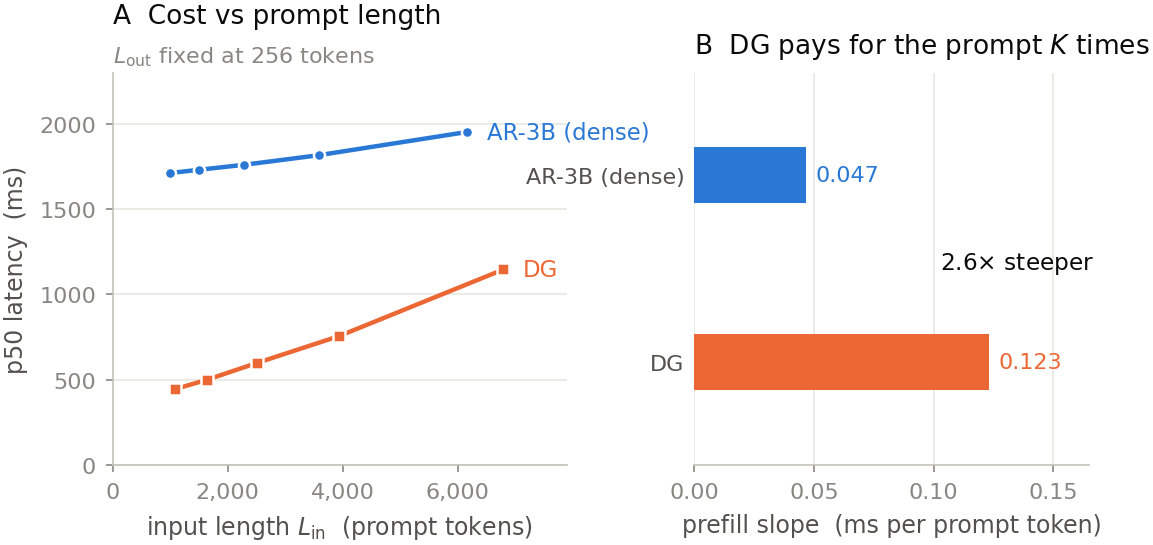
\includegraphics[width=\linewidth]{figures/fig3_input_sweep.png}
\caption{Input-length sweep at fixed $L_{\mathrm{out}}{=}\canvasLength$
(BGL, $n{=}100$; AR arm is dense AR-3B). The prompt is lengthened by
repeating the schema block, so the task is unchanged.}
\label{fig:input}
\end{figure}

\subsection{A free Pareto improvement at canvas $= 128$}

At canvas $=128$ the base falls to \canvasOneTwentyEightBase\,ms
($-2.0\%$) \emph{and} 9-field F1 rises to
\canvasOneTwentyEightFone{}, an improvement on both axes
simultaneously. At canvas $=64$ the base rises $48\%$ because the
per-canvas fixed overhead is paid twice as often; that setting is not
viable. Block size, not denoising schedule, is the interesting design
variable. Canvas $=128$ barely moves the crossover, $L^{*}$ falls
from $48$ to $46$ tokens, because the base drops only $2\%$, but
canvas $=64$ pushes it to $L^{*}\approx73$, since $L^{*}$ scales with
the base and that base is $48\%$ higher. Shrinking the canvas doesn't
shrink the prefill it must re-attend, so a smaller canvas buys
finer-grained output at the cost of paying the fixed overhead more
often.

\subsection{Joint canvas$\times$K sweep confirms canvas $= 128$ is
Pareto-optimal}

A full $4\times5$ grid (canvas $\in \{64,128,256,512\}$, $K \in
\{2,4,8,16,32\}$, $n{=}200$ per cell) confirms the single-knob finding
holds across all $K$ values, not just $K{=}8$. The Pareto frontier
contains six cells; the paper's current operating point (canvas$=256$,
$K{=}8$: p50$=$376\,ms, F1$=$0.853) is \emph{dominated} by
(canvas$=128$, $K{=}8$: p50$=$368\,ms, F1$=$0.864), which is faster
and higher quality simultaneously. The $K$ knee also shifts left at
smaller canvas: at canvas$=128$, $K{=}8$ is near saturation
(F1$=$0.864), while at canvas$=256$ quality keeps improving through
$K{=}32$ (F1$=$0.862). Canvas$=64$ remains non-viable even at $K{=}32$
(F1$=$0.834, below the canvas$=256$ $K{=}8$ baseline). Full data in
\texttt{results/issue114\_joint\_sweep.json}.

\section{Quality vs output length}
\label{app:quality}

The diffusion model degrades gracefully against a \emph{time} budget
and catastrophically against an \emph{output-length} budget. At
$L{=}128$ the AR model retains \arFOneTwentyEight{} F1 and
\arValidTwentyEight\% schema validity, while the diffusion model falls
to \dgFOneTwentyEight{} and \dgValidTwentyEight\%. Which budget an
application faces decides which architecture is safer.

\begin{figure}[t]
\centering
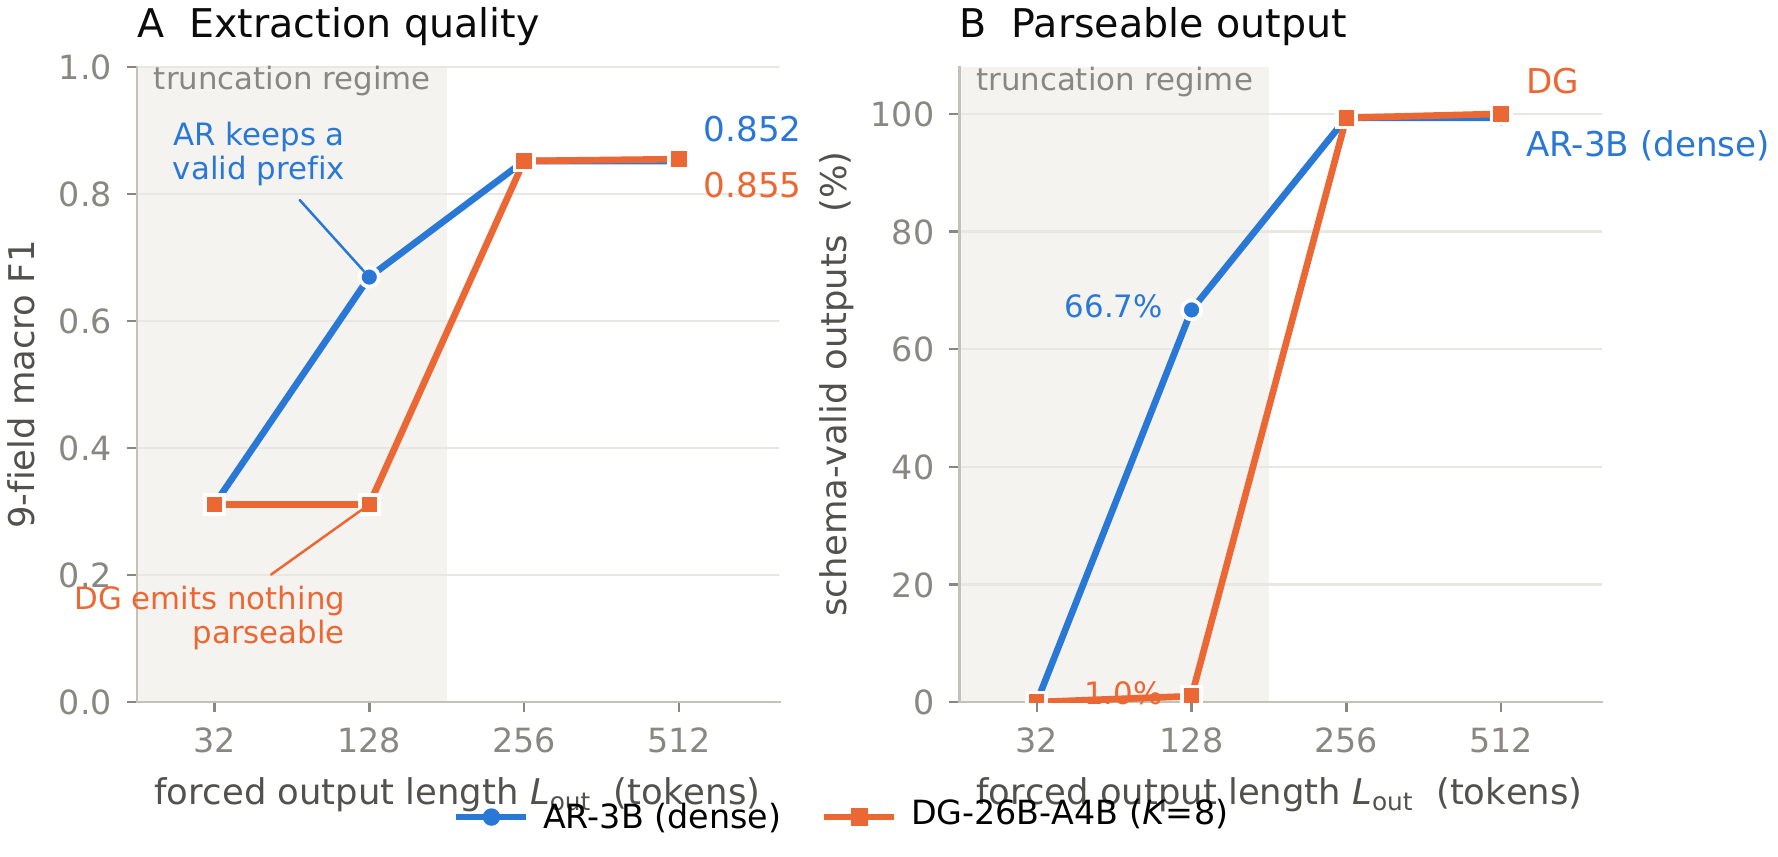
\includegraphics[width=\linewidth]{figures/fig5_quality_vs_length_hires.png}
\caption{Quality and schema validity vs forced output length (BGL,
$n{=}300$; AR arm is dense AR-3B). The diffusion model's quality rises
with $L$ and plateaus; AR-3B F1 is flat from $L{=}256$ to $L{=}512$
because first-object-wins parsing discards the rambled continuation.}
\label{fig:quality}
\end{figure}

\section{Latency distributions}
\label{app:distributions}

The per-event latency distributions are asymmetric. Across 300 events at
$L{=}\canvasLength$:
\begin{itemize}[nosep]
\item AR-3B (dense baseline) per-event CV: \arEventCV\%; max/median: \arMaxMed$\times$.
\item DG-26B-A4B per-event CV: \dgEventCV\%; max/median: \dgMaxMed$\times$.
\end{itemize}
AR's \arEventCV\% CV means its p50 is a reliable planning number;
the DG arm's \dgEventCV\% means a p99 SLA lands in a very different
place than p50 would suggest.

\section{Does the advantage survive natural long output?}
\label{app:forced}

Table~\ref{tab:niche} lets AR-30B stop at its natural EOS near 123
tokens, so its long-output rows are a plateau rather than a
measurement of long output; neither arm is forced there. The question
this appendix answers is what happens when the \emph{task} makes the
output long. A multi-record extraction task --- emit a JSON array of
$N$ structured records from $N$ consecutive log lines --- produces
output of roughly $N \times 140$ tokens naturally, without forcing.
A record inside an array costs slightly more than the 123 tokens of a
bare record, for the enclosing punctuation and indentation.
Table~\ref{tab:forced} applies the fitted cost laws
(Eqs.~\ref{eq:ar}--\ref{eq:dg}):

\begin{table}[ht!]
\centering
\caption{What the cost laws predict when the task itself makes output
long. Row 1 is measured; rows 2--4 apply Eqs.~\ref{eq:ar}--\ref{eq:dg}
at the natural output length of an $N$-record extraction. The
advantage grows rather than narrows here --- the opposite of
Table~\ref{tab:niche} --- because AR is no longer stopped by EOS at
123 tokens, so its line keeps climbing while DG adds one bounded
canvas at a time.}
\label{tab:forced}
\begin{tabular}{@{}lrrrr@{}}
\toprule
Task & $L_{\mathrm{out}}$ & AR-30B (ms) & DG (ms) & Ratio \\
\midrule
Single record (unforced) & 123 & 5899 & 379 & DG $15.6\times$ \\
Multi-record $N{=}2$ & 280 & 13435 & 498 & DG $27.0\times$ \\
Multi-record $N{=}4$ & 560 & 26791 & 618 & DG $43.4\times$ \\
Multi-record $N{=}8$ & 1120 & 53503 & 857 & DG $62.4\times$ \\
\bottomrule
\end{tabular}
\end{table}

So the eightfold figure quoted in the abstract is the conservative
reading, not the optimistic one: it describes AR at its natural output
length. When the task genuinely demands a thousand tokens, the
staircase pulls further ahead, not less.

\section{Why the batching ceiling is likely architectural}
\label{app:batching_architectural} The diffusion batching ceiling ($\leq 1.7\times$) is measured on two
engine-bounded stacks (Appendix~\ref{app:batching}). We argue here that
the ceiling is likely architectural, not an engine bug, by reasoning
about the mechanism. \paragraph{The KV-cache reuse argument.}
Autoregressive batching is cheap because of KV-cache reuse: when two
requests share a prompt prefix, the prefill is computed once and the KV
cache is shared. Even without prefix sharing, each request's KV cache
persists across decode steps, so the GPU alternates between requests at
low marginal cost per token. Block-diffusion invalidates both forms of reuse: \begin{enumerate}[nosep]
\item \textbf{Cross-request prefix sharing} requires that both requests
are at the same denoising step. Even if vLLM's mixed-phase crash were
fixed, requests at different $K$ steps cannot share a KV cache because
the attention mask differs per step.
\item \textbf{Within-request KV persistence} across denoising steps
fails because the denoising tokens' KV changes at every step (the mask
changes), so the per-step computation cannot reuse the previous step's
activations for the denoising positions.
\end{enumerate} The net effect: each denoising step is a fresh forward pass over the full
sequence (prompt + denoising positions), with a different attention mask.
The GPU does the same FLOPs whether batching or not, because the
attention pattern is request-specific and step-specific. This is
structurally different from AR decoding, where the attention pattern is
causal and the KV cache grows monotonically. Disabling prefix caching on
the AR arm drops its multiplier from $\cacheOnMult\times$ to
$\cacheOffMult\times$ --- still more than twenty times the diffusion
ceiling. A patched vLLM might raise the DG multiplier to $\sim 2$--$3\times$,
still an order of magnitude below AR. This is a structural argument, not
a measurement.


\end{document}
